\documentclass{article}
\usepackage{graphicx} % Required for inserting images

\title{An Evolutionary Approach to the Maximum K-Colorable Subgraph Problem}
\author{James Kyle Harrison}
\date{April 2nd, 2023}

\begin{document}

\maketitle

\section{Introduction}
 \hspace{\parindent} One of the most important branches of algorithmic research over the past century has been in Graph Theory. Many of the problems dissected within graph theory are quite old, and have had many algorithms that have been created to efficiently solve these problems. Although solutions have been created for these types of problems, these solutions require searching through a vast array of potential solutions before deciding on one. That is to say, that although old solutions have been made, newer technologies and approaches can come along and change what is observed to be an efficient solution. What was once considered to be the optimal solution in older algorithms could in fact be a local optimal solution that does not compare with what is considered the current local optimal solutions. We have moved beyond the days of straightforward greedy algorithms and have moved to an era of various self-learning algorithms, such as evolutionary algorithms, that are able to give much better results over the course of several learning cycles.
 \par A problem that this can be observed in is the Maximum k-Colorable Subgraph Problem (MkCS), a well known problem in graph theory. In this problem, one is given an undirected graph $ G = (V,E)$ and an integer 'k'. The objective is to find the largest subset of nodes in the graph such that induced subgraph G[V'] is k-colorable, or in simpler terms, to color a graph using k-different colors such that no two adjacent vertices have the same color. Unlike most graph theory problems (such as the k-partite problem), the MkCS problem does not necessarily have the goal of filling the entire graph, but more or less fill as much as possible of the nodes in a graph using these 'k' distinct colors. This problem is commonly mistaken with the generic Graph Coloring problem (where one determines if an entire graph can be colored with k-colors) as if the Maximum K-Colorable Subgraph is the entire graph then they both give the same result, and also has plenty of overlap with many topics in graphy theory.
 \par This literature review will go over the history of the Maximum k-Colorable Subgraph Problem in regards to the early history and the approaches taken towards this problem in regards to evolutionary algorithms. The latter half of this document will then describe the design of these evolutionary algorithms to help develop our own algorithm to effectively tackle this problem.
 \section{Historical Development of MkCS}
 \hspace{\parindent} As previously described, the Maximum k-Colorable Problem is the problem of determining the largest set of vertices of the graph that can be colored using k different colors such that no adjacent vertices share the same color [8], and was proven to be NP-hard on circular undirected graphs where k is greater than 2 (and NP-Complete when k is less than or equal to 2) by Lovasz's Sandwich Theorem [6] to define two general efficient bounds created through difficult functional calculations. Although it is impossible to generalize the performance of an approach to the MkCS problem, we do know that through the proofs of Narasimhan [6] that we can expect the processing and subgraph of greedy and sudo-greedy approaches to increase at a nearly steady of rate of 4/3 as the amount of nodes in the graph increases, and the effectiveness continues to decrease the greater the k involved. Even in cases where we allow the greedy approaches to use multiple of their best results, these solutions are closer to the worst case subsets than the optimal subset [4]. 
 \par Although the Maximum k-Colorable Problem is an old problem, approximations for the bounds of this problem have changed quite a bit over time with the development of more complicated solutions. These approximations over time have pushed closer to what has been seen with the approximations of Campelo and Correa, as well as Januschowski and Pfetsch [5], where the 'possible color symmetry' of the graph is taken into consideration for the approximation as highly symmetrical graphs have a more solid bounds, however that still does not help in solidifying anything for this problem as more sophisticated and thoroughly connected graphs makes defining the symmetry of these graphs a problem in it's own right. As it stands, not only is the problem an NP-Hard but approximating for this problem is also considered NP-Hard [3].
 
 \section{Evolutionary Approaches}
  \hspace{\parindent} As previously described, the Maximum k-Colorable Subgraph Problem has a long history of approaches to it, however when it comes to evolutionary approaches it can be quite difficult to not only find comparable algorithms due to the complexity and entirely different data sets used to test their performance. There are however graph theory problems that overlap with the Maximum k-Colorable Subgraph Problem to a degree which allows for a comparison to help create a better performing algorithm, such as the Maximum Bipartite Subgraph Problem and the Maximum k-Cut Problem. Although this is the case, for the sake of honing in on understanding how to develop for this particular problem we will be reviewing only evolutionary approaches to graph coloring.
  \par The earliest approach that can be compared to an evolutionary approach in attempting the MkCS Problem is DSatur created by Daniel Brélaz in 1979 [1] which combined principles of both greedy and evolutionary models by using the amount of adjacent different colors to greedily color nodes with the possibility of random selection in the case of a tie in these node it is deciding to color. This approach also was expected to run multiples times such that useful statistics could be created, but as time went on this model was eventually modified to be able to run a form of backtracking to look at more possibilities before making a node and color selection.
   \begin{figure}
    \centering
    \caption{}
    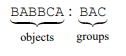
\includegraphics[scale=1.2]{ex1.png}
   \end{figure}
  \par About a decade after DSatur, an explosion of genetic algorithmic research began in practically all problems in graph theory, and with that two main evolutionary approaches to the MkCS Problem came to be: Grouping Genetic Algorithms and Standard Genetic Algorithms. The Grouping Genetic Algorithm (developed by Emaneul Falkenauer in 1992) is a type of genetic algorithm that is specialized in taking on problems that require a particular structure or grouping to be formed to create a local optimum solution [2], which clearly has it's benefits in this problem as the groupings can be easily made from the k-colors. In particular, a grouping genetic model created by Eiben, Hauw, and Hemert for the MkCS Problem will have the nodes be the 'object genes' for the color groupings. Figure 1 helps describe what this means by taking a look at an individual where the nodes in our graph is (N=)6 and  groupings created is (K=)3, where the groupings are the potential colors of B, A, and C and the objects list is the nodes coloring order (N1-B, N2-A, N3-B, etc.). The grouping structure is then used in tandem with three common genetic operators: crossover, mutation, and inversion. The algorithm first begins by initializing the population by starting at a random node and colouring the rest. The population is then filtered by using a 2-Tournament Selection to pit two random individuals against each other and removing the loser (one with worst fitness) from the population and added to a list. The tournaments continue until the list is in the order of the worst fitness individuals being at the bottom and the best at the top. Then the crossover function starts, which would take 2 individuals structured like Figure 1, and select two random crossing points in the groups to injects its contents into the section between these crossing points. This in result injects information from Parent 1 into Child 2, while Child 1 continues to remain the same as Parent 1, and will then move from doing so for the groupings into the objects. Continuing on in the crossover function, once Child 2 has been injected any empty groupings will be removed resulting in objects to lose assigned values. These particular objects locations are then stored in a queue, which reinsert objects into the queue through a first-fit heuristic on a random set of colors. If there is not any colors possible, it then creates a new group and assigns remaining objects to this group which in certain scenarios this can lead to a significant increase in memory usage, and in term processing speed. The crossover function will then move on to doing the same for Parent 2 being the primary injector. The mutation function of this grouping genetic algorithm will then work in a similar manner by deleting elements in the group of an individual and then unassigning colors for objects effected and then reinsert nodes using the first-fit heuristic that was in the crossover. The final operator, inversion, only uses the groups of an individual and will again mark two random points and will invert the order of the groups between said points. Fitness of the population in the model is the amount of nodes in each color that does not have as many nodes as the color with at least the third most nodes (ex:  if color A, B, and C had 6 nodes colored and nodes D and E had 5, the fitness would be 2). Eiben, Hauw, and Hemert describe this fitness function as: 
  \begin{equation}
       F_{k}(x) = l - k + \sum_{i=k+1}^l g(x, c_{i})
  \end{equation}
  where k is the colors used, k $\le$ l and l is the amount of colors, i increments from 1 to l, and the graph g(x, $c_{i}$) occurs in an order such that each incremented child has a fitness less than or equal to the proceeding child. Figure 2 helps define the general layout of this algorithm, with the population being set to 50, crossover rate of .24, and a mutation and inversion rate of .08.
  \begin{figure}
    \centering
    \caption{}
    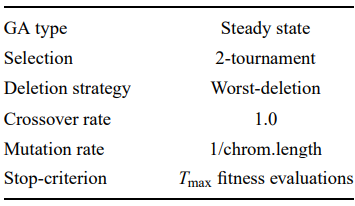
\includegraphics[scale=.6]{ex3.png}
   \end{figure}
 \par The results of the grouping genetic model will be discussed in the next session, however we should also look at the strengths of more standard genetic models to better understand the overall structure and workflow of genetic models as typically the majority of these will be nearly identical. The work of Hindi and Yampolski [3] helps demonstrate this by defining a default generational genetic algorithm for the Maximum k-Colorable Subgraph Problem and then creates a model to improve upon through a few different modifications. Starting with the default algorithm, it begins by selecting a population of chromosomes randomly, and continuously have the better parents create superior offspring until a certain amount of generations has been reached via a generic crossover and mutation operator. The population size is always the same, and the bottom half in performance in the population are replaced with new random chromosomes. Hindi and Yampolski then go on to explain that additional methods and modifying these traditional methods we can improve this, as this default generational genetic algorithm will not be able to handle or even compare to the global optimum solution in complex undirected graphs. The particular improvements used in their approach was to have two different parent selection functions, a near identical crossover function, and two different mutation functions as well. The two separate selection and mutation functions are called in separate situations depending on the best fitness in the population; if the best fitness is greater than 4 then parentSelection1 and mutation1 and called and if it is less than parentSelection2 and mutation2 will be selected. By using two different algorithms, they were able to increase the amount of local optimal solution that it is able to discover while also decreasing runtime. The reasoning for this is best described by the condition to choose which one to use, the fitness value being greater or less than 4. As previously described, graph theory is a very complicated topic for research as different data sets will give different results, and these data sets can change from the amount of nodes, to the amount of edges, and of course for our problem the k-colors. Therefore, by having two separate algorithms for selection and mutation, we are able to use an algorithm that works more consistently for smaller (or less connected) data sets and also have an algorithm for larger data sets. Crossover is nearly identical in this model to what was considered a generic approach by randomly selecting a point in the individual and injecting information from everything to that point in to the individual, and everything beyond that is injected from parent 2. The last part of their implementation is a 'Wisdom of Crowds' function, which is used to find a best-fit solution in the case that the algorithm can not find an optimal solution after the defined amount of generations. 
\begin{figure}
    \centering
    \caption{}
    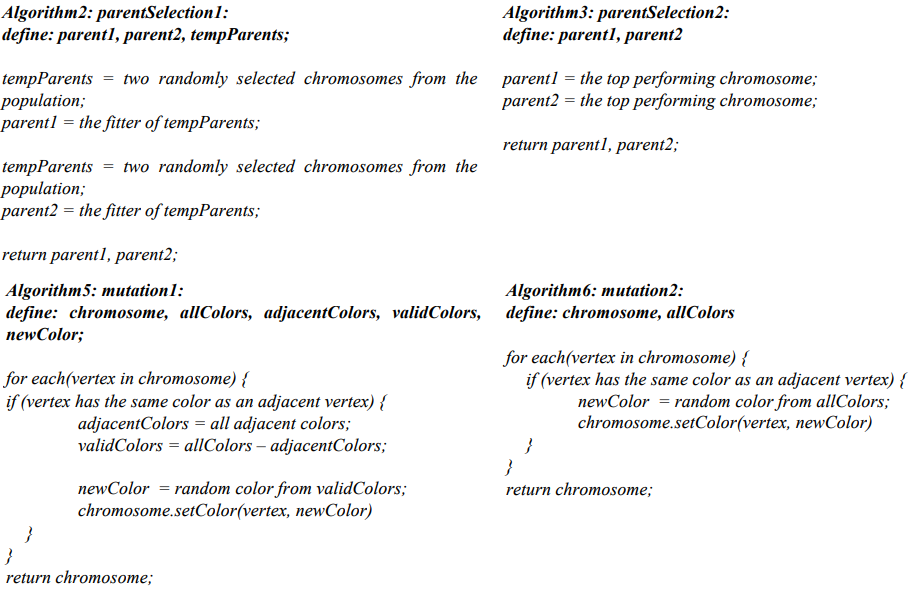
\includegraphics[scale=.5]{algo.png}
   \end{figure}
 \section{Comparison}
    \hspace{\parindent} Although these genetic approaches were all developed for the same purpose the strengths of each one can be hard to pinpoint as just from the surface they can be seen as drastically similar. Of course the overall algorithms themselves are not what change, but instead the operators that are used between them. We can see with an implementation such as the Hindi and Yampolskiy's implementation that having multiple of the same type of operator is especially handy in guiding one to better results from the population. The grouping genertic algorithm described by Eiben, Hauw, and Hemert however also highlights that when creating a new population it is important to keep some of the best from the previous generation through a form of tournament selection to keep a larger amount of local global maximums to be discover-able. Tournament selection is also quite handy when it comes to handling noisy or imperfect fitness functions, thus it is a safe selection when attempting to minimize potential 'noise' in the algorithm [7]. If there's one main difference between these form of genetic algorithms it comes down to the functionality of the crossover, where grouping in the grouping genetic algorithm has the majority of it's function. As documented by the detailing of this grouping algorithm, having two points to dictate limits on crossover helps create more diverse solutions at the cost of having to duplicate processing for splitting and handling the object and groupings. This type of crossover does seem to have some benefit, however a potential best solution for a crossover to take from both of these solutions is to instead follow Hindi and Yampolskiy's crossover but instead with a 2-point crossover, where one could gain the benefits of the grouping algorithm while slightly minimizing memory usage.
 \section{Conclusion}
    \hspace{\parindent} We have examined the strengths of a couple of genetic solutions when compared to a standard generational genetic algorithm to the Maximum k-Colorable Subgraph Problem, and also identified the similarities in not only the design of these solutions, but the incredible similarities of designing solutions in general in evolutionary approaches. With this information, one can have a better understanding of what meets the bare minimum requirements of creating an evolutionary algorithm, as well as how to improve upon it and how important the data sets that will be are to improving upon an genetic algorithm. For algorithms that require running data sets of vastly different sizes providing multiple functions of traditional genetic algorithm. The approaches described here may not be the most advanced solutions, and potentially may not give what is considered the most optimal solutions for the standards of 2023, but they outline the potential of evolutionary approaches quite well.
 \section{References}
    \begin{itemize}
        \item [1] Brélaz, Daniel (1979-04-01). "New methods to color the vertices of a graph". Communications of the ACM. 22 (4): 251–256. doi:10.1145/359094.359101. ISSN 0001-0782. S2CID 14838769.
        \item [2] Eiben, Hauw, and Hemert. (1998) "Graph Coloring with Adaptive Evolutionary Algorithms", Leiden University - Journal of Heuristics
        \\https://www.cs.vu.nl/~gusz/papers/Graph\%20\\Coloring\%20with\%20Adaptive\%20Evolutionary\%20Algorithms.pdf
        \item [3] Hindi and Yampolskiy (2012). "Genetic Algorithm Applied to the Graph Coloring Problem" J.B. School of Engineering \\https://ceur-ws.org/Vol-841/submission\textunderscore10.pdf
        \item [4] Hochbaum, Dorit S, and Anu Pathria. “Analysis of the Greedy Approach in Problems of Maximum k-Coverage.” University of California, Berkeley Research, 9 Mar. 1998, https://hochbaum.ieor.berkeley.edu/html/pub/HPathria-max-k-coverage-greedy.pdf. 
        \item [5] Januschowski, Tim, and Marc E Pfetsch. “The Maximum k-Colorable Subgraph Problem and Orbitopes.” Science Direct - Elsevier, 26 May 2011, https://www.sciencedirect.com/science/article/pii/S1572528611000272. 
        \item [6] Lovasz, L., An Algorithmic Theory of Numbers, Graphs, and Convexity, \\
        CBMS 50, SIAM, Philadelphia, 1986.\\ https://doc.lagout.org/science/0\textunderscore Computer\%20Science/2\textunderscore \\ Algorithms/An\%20Algorithmic\%20Theory\\\%20of\%20Numbers,\%20Graphs\%20and\%20Convexity\%20\%5BLov\%C3\%A1sz\%201987-01-01\%5D.pdf
        \item [7] Miller and Goldberg (2005) "Genetic Algorithms, Tournament Selection, and the Effects of Noise" Complex Systems 9, 193-212, \\ https://wpmedia.wolfram.com/uploads/sites/13/2018/02/09-3-2.pdf
        \item [8] Narasimhan, Giri. “The Maximum K-Colorable Subgraph Problem.” University of Wisconsin Research, https://research.cs.wisc.edu/techreports/viewreport.php?report=864. 
        \item [9] Olga et al, "The Maximum k-colorable subgraph problem and related problems", Arxiv,  https://arxiv.org/pdf/2001.09644.pdf
    \end{itemize}
\end{document}
